\documentclass{standalone}
\usepackage{tikz}
\usetikzlibrary{patterns, positioning}
\usepackage[sfdefault]{ClearSans} %% option 'sfdefault' activates Clear Sans as the default text font
\usepackage[T1]{fontenc}

\begin{document}
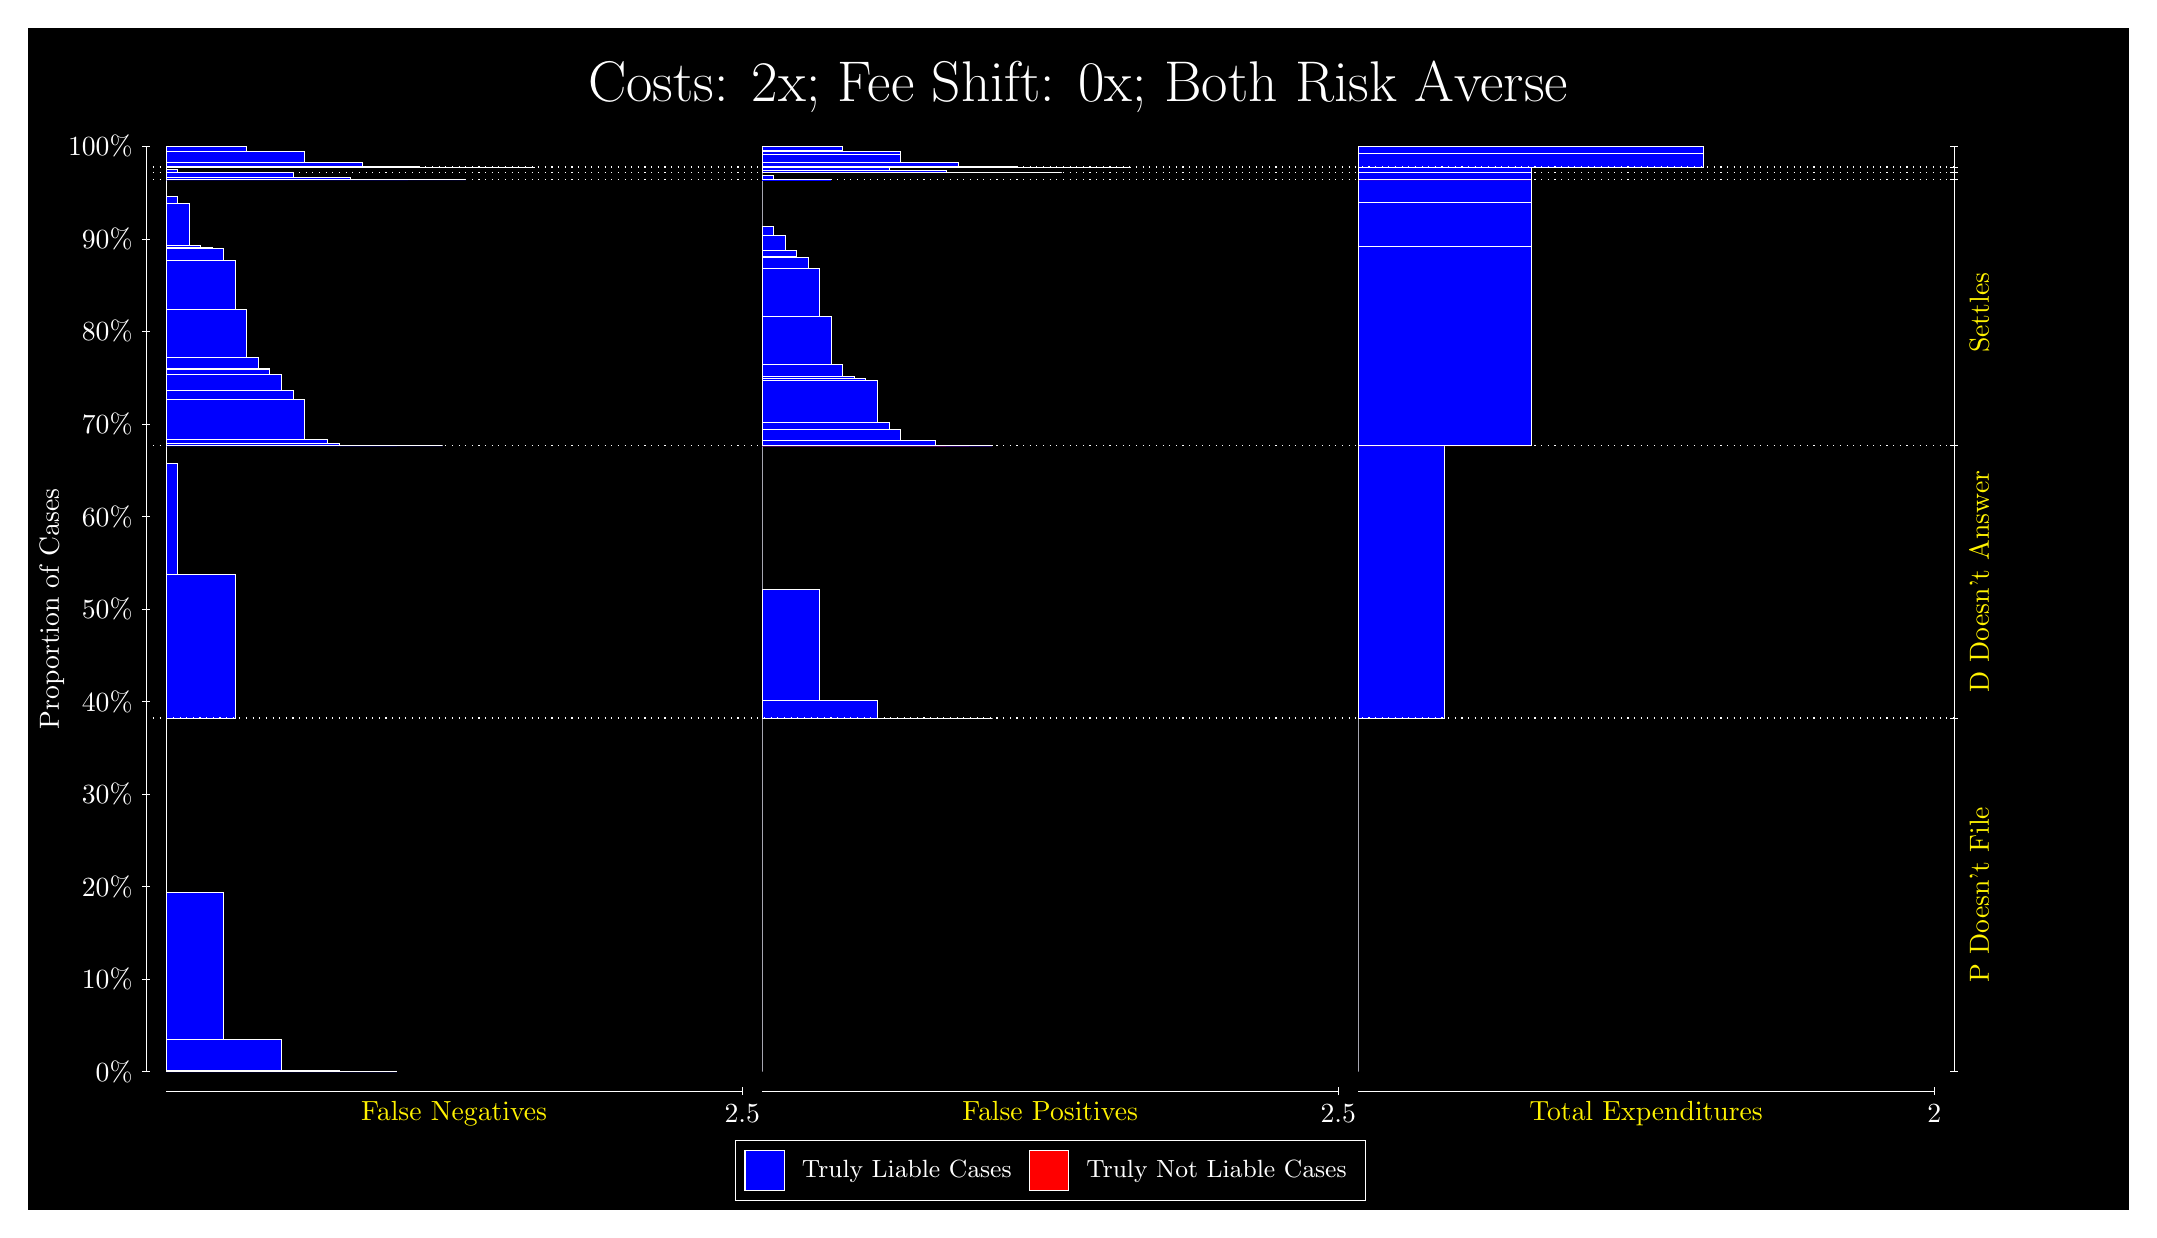
\begin{tikzpicture}
\draw[fill=black] (0,0) rectangle (26.667,15);
\draw[text=white] (0,13.5) rectangle (26.667,15) node[midway] {\huge Costs: 2x; Fee Shift: 0x; Both Risk Averse};
\draw[white, very thin] (1.5,1.75) -- (1.5,13.5);
\node[rotate=90, text=white, anchor=center] at (0.3, 7.625) {Proportion of Cases};
\draw[white, very thin] (1.45,1.75) -- (1.55,1.75);
\node[text=white, anchor=east] at (1.45, 1.75) {0\%};
\draw[white, very thin] (1.45,2.925) -- (1.55,2.925);
\node[text=white, anchor=east] at (1.45, 2.925) {10\%};
\draw[white, very thin] (1.45,4.1) -- (1.55,4.1);
\node[text=white, anchor=east] at (1.45, 4.1) {20\%};
\draw[white, very thin] (1.45,5.275) -- (1.55,5.275);
\node[text=white, anchor=east] at (1.45, 5.275) {30\%};
\draw[white, very thin] (1.45,6.45) -- (1.55,6.45);
\node[text=white, anchor=east] at (1.45, 6.45) {40\%};
\draw[white, very thin] (1.45,7.625) -- (1.55,7.625);
\node[text=white, anchor=east] at (1.45, 7.625) {50\%};
\draw[white, very thin] (1.45,8.8) -- (1.55,8.8);
\node[text=white, anchor=east] at (1.45, 8.8) {60\%};
\draw[white, very thin] (1.45,9.975) -- (1.55,9.975);
\node[text=white, anchor=east] at (1.45, 9.975) {70\%};
\draw[white, very thin] (1.45,11.15) -- (1.55,11.15);
\node[text=white, anchor=east] at (1.45, 11.15) {80\%};
\draw[white, very thin] (1.45,12.325) -- (1.55,12.325);
\node[text=white, anchor=east] at (1.45, 12.325) {90\%};
\draw[white, very thin] (1.45,13.5) -- (1.55,13.5);
\node[text=white, anchor=east] at (1.45, 13.5) {100\%};

\draw[white, very thin] (24.457,1.75) -- (24.457,13.5);
\draw[white, very thin] (24.407,1.75) -- (24.507,1.75);
\node[anchor=west] at (24.407, 1.75) {};
\draw[white, very thin] (24.407,6.2402) -- (24.507,6.2402);
\node[anchor=west] at (24.407, 6.2402) {};
\draw[white, very thin] (24.407,9.7002) -- (24.507,9.7002);
\node[anchor=west] at (24.407, 9.7002) {};
\draw[white, very thin] (24.407,13.076) -- (24.507,13.076);
\node[anchor=west] at (24.407, 13.076) {};
\draw[white, very thin] (24.407,13.173) -- (24.507,13.173);
\node[anchor=west] at (24.407, 13.173) {};
\draw[white, very thin] (24.407,13.238) -- (24.507,13.238);
\node[anchor=west] at (24.407, 13.238) {};
\draw[white, very thin] (24.407,13.5) -- (24.507,13.5);
\node[anchor=west] at (24.407, 13.5) {};

\draw[white, very thin, fill=blue] (1.75,1.75) rectangle (4.6775,1.7501);
\draw[white, very thin, fill=blue] (1.75,1.7501) rectangle (3.9457,1.7637);
\draw[white, very thin, fill=blue] (1.75,1.7637) rectangle (3.2138,2.1608);
\draw[white, very thin, fill=blue] (1.75,2.1608) rectangle (2.4819,4.0318);
\draw[white, very thin, fill=red] (1.75,4.0318) rectangle (1.75,4.0318);
\draw[white, very thin, fill=blue] (1.75,4.0318) rectangle (1.75,6.2402);
\draw[white, very thin, fill=blue] (1.75,6.2402) rectangle (2.6283,8.0648);
\draw[white, very thin, fill=blue] (1.75,8.0648) rectangle (1.8964,9.4707);
\draw[white, very thin, fill=red] (1.75,9.4707) rectangle (1.75,9.4707);
\draw[white, very thin, fill=blue] (1.75,9.4707) rectangle (1.75,9.7002);
\draw[white, very thin, fill=blue] (1.75,9.7002) rectangle (5.2631,9.7002);
\draw[white, very thin, fill=blue] (1.75,9.7002) rectangle (4.6775,9.7003);
\draw[white, very thin, fill=blue] (1.75,9.7003) rectangle (4.5312,9.7015);
\draw[white, very thin, fill=blue] (1.75,9.7015) rectangle (4.3848,9.7015);
\draw[white, very thin, fill=blue] (1.75,9.7015) rectangle (4.092,9.7018);
\draw[white, very thin, fill=blue] (1.75,9.7018) rectangle (3.9457,9.7284);
\draw[white, very thin, fill=blue] (1.75,9.7284) rectangle (3.7993,9.7765);
\draw[white, very thin, fill=blue] (1.75,9.7765) rectangle (3.6529,9.7834);
\draw[white, very thin, fill=blue] (1.75,9.7834) rectangle (3.5065,10.289);
\draw[white, very thin, fill=blue] (1.75,10.289) rectangle (3.3602,10.401);
\draw[white, very thin, fill=blue] (1.75,10.401) rectangle (3.2138,10.601);
\draw[white, very thin, fill=blue] (1.75,10.601) rectangle (3.0674,10.671);
\draw[white, very thin, fill=blue] (1.75,10.671) rectangle (3.0674,10.682);
\draw[white, very thin, fill=blue] (1.75,10.682) rectangle (2.921,10.826);
\draw[white, very thin, fill=blue] (1.75,10.826) rectangle (2.7746,11.43);
\draw[white, very thin, fill=blue] (1.75,11.43) rectangle (2.6283,12.047);
\draw[white, very thin, fill=blue] (1.75,12.047) rectangle (2.4819,12.2);
\draw[white, very thin, fill=blue] (1.75,12.2) rectangle (2.3355,12.217);
\draw[white, very thin, fill=blue] (1.75,12.217) rectangle (2.3355,12.217);
\draw[white, very thin, fill=blue] (1.75,12.217) rectangle (2.1891,12.242);
\draw[white, very thin, fill=blue] (1.75,12.242) rectangle (2.0428,12.778);
\draw[white, very thin, fill=blue] (1.75,12.778) rectangle (1.8964,12.871);
\draw[white, very thin, fill=red] (1.75,12.871) rectangle (1.75,12.871);
\draw[white, very thin, fill=blue] (1.75,12.871) rectangle (1.75,13.076);
\draw[white, very thin, fill=blue] (1.75,13.076) rectangle (5.5558,13.076);
\draw[white, very thin, fill=blue] (1.75,13.076) rectangle (4.8239,13.076);
\draw[white, very thin, fill=blue] (1.75,13.076) rectangle (4.092,13.113);
\draw[white, very thin, fill=blue] (1.75,13.113) rectangle (3.3602,13.172);
\draw[white, very thin, fill=blue] (1.75,13.172) rectangle (2.6283,13.173);
\draw[white, very thin, fill=red] (1.75,13.173) rectangle (1.75,13.173);
\draw[white, very thin, fill=blue] (1.75,13.173) rectangle (2.6283,13.174);
\draw[white, very thin, fill=blue] (1.75,13.174) rectangle (1.8964,13.214);
\draw[white, very thin, fill=red] (1.75,13.214) rectangle (1.75,13.214);
\draw[white, very thin, fill=blue] (1.75,13.214) rectangle (1.75,13.238);
\draw[white, very thin, fill=blue] (1.75,13.238) rectangle (6.4341,13.238);
\draw[white, very thin, fill=blue] (1.75,13.238) rectangle (5.7022,13.238);
\draw[white, very thin, fill=blue] (1.75,13.238) rectangle (4.9703,13.242);
\draw[white, very thin, fill=blue] (1.75,13.242) rectangle (4.2384,13.303);
\draw[white, very thin, fill=blue] (1.75,13.303) rectangle (3.5065,13.435);
\draw[white, very thin, fill=blue] (1.75,13.435) rectangle (2.7746,13.496);
\draw[white, very thin, fill=blue] (1.75,13.496) rectangle (2.0428,13.5);
\draw[white, very thin, fill=red] (1.75,13.5) rectangle (1.75,13.5);
\draw[white, very thin, fill=blue] (1.75,13.5) rectangle (1.75,13.5);
\draw[white, very thin, fill=red] (9.3189,1.75) rectangle (9.3189,1.75);
\draw[white, very thin, fill=blue] (9.3189,1.75) rectangle (9.3189,6.2402);
\draw[white, very thin, fill=red] (9.3189,6.2402) rectangle (12.246,6.2402);
\draw[white, very thin, fill=blue] (9.3189,6.2402) rectangle (12.246,6.2402);
\draw[white, very thin, fill=blue] (9.3189,6.2402) rectangle (11.515,6.2412);
\draw[white, very thin, fill=blue] (9.3189,6.2412) rectangle (10.783,6.4696);
\draw[white, very thin, fill=blue] (9.3189,6.4696) rectangle (10.051,7.8756);
\draw[white, very thin, fill=blue] (9.3189,7.8756) rectangle (9.3189,9.7002);
\draw[white, very thin, fill=red] (9.3189,9.7002) rectangle (12.246,9.7002);
\draw[white, very thin, fill=blue] (9.3189,9.7002) rectangle (12.246,9.7004);
\draw[white, very thin, fill=red] (9.3189,9.7004) rectangle (11.954,9.7004);
\draw[white, very thin, fill=blue] (9.3189,9.7004) rectangle (11.954,9.7004);
\draw[white, very thin, fill=red] (9.3189,9.7004) rectangle (11.661,9.7004);
\draw[white, very thin, fill=blue] (9.3189,9.7004) rectangle (11.661,9.7006);
\draw[white, very thin, fill=blue] (9.3189,9.7006) rectangle (11.515,9.7674);
\draw[white, very thin, fill=red] (9.3189,9.7674) rectangle (11.368,9.7674);
\draw[white, very thin, fill=blue] (9.3189,9.7674) rectangle (11.368,9.7676);
\draw[white, very thin, fill=blue] (9.3189,9.7676) rectangle (11.222,9.7676);
\draw[white, very thin, fill=red] (9.3189,9.7676) rectangle (11.075,9.7676);
\draw[white, very thin, fill=blue] (9.3189,9.7676) rectangle (11.075,9.9057);
\draw[white, very thin, fill=blue] (9.3189,9.9057) rectangle (10.929,9.9989);
\draw[white, very thin, fill=blue] (9.3189,9.9989) rectangle (10.783,10.534);
\draw[white, very thin, fill=blue] (9.3189,10.534) rectangle (10.636,10.56);
\draw[white, very thin, fill=red] (9.3189,10.56) rectangle (10.49,10.56);
\draw[white, very thin, fill=blue] (9.3189,10.56) rectangle (10.49,10.56);
\draw[white, very thin, fill=blue] (9.3189,10.56) rectangle (10.49,10.577);
\draw[white, very thin, fill=blue] (9.3189,10.577) rectangle (10.344,10.729);
\draw[white, very thin, fill=blue] (9.3189,10.729) rectangle (10.197,11.347);
\draw[white, very thin, fill=blue] (9.3189,11.347) rectangle (10.051,11.951);
\draw[white, very thin, fill=blue] (9.3189,11.951) rectangle (9.9044,12.095);
\draw[white, very thin, fill=blue] (9.3189,12.095) rectangle (9.758,12.105);
\draw[white, very thin, fill=blue] (9.3189,12.105) rectangle (9.758,12.176);
\draw[white, very thin, fill=blue] (9.3189,12.176) rectangle (9.6116,12.375);
\draw[white, very thin, fill=blue] (9.3189,12.375) rectangle (9.4652,12.488);
\draw[white, very thin, fill=blue] (9.3189,12.488) rectangle (9.3189,13.076);
\draw[white, very thin, fill=red] (9.3189,13.076) rectangle (10.197,13.076);
\draw[white, very thin, fill=blue] (9.3189,13.076) rectangle (10.197,13.078);
\draw[white, very thin, fill=blue] (9.3189,13.078) rectangle (9.4652,13.137);
\draw[white, very thin, fill=blue] (9.3189,13.137) rectangle (9.3189,13.173);
\draw[white, very thin, fill=red] (9.3189,13.173) rectangle (13.125,13.173);
\draw[white, very thin, fill=blue] (9.3189,13.173) rectangle (13.125,13.173);
\draw[white, very thin, fill=blue] (9.3189,13.173) rectangle (12.393,13.173);
\draw[white, very thin, fill=blue] (9.3189,13.173) rectangle (11.661,13.197);
\draw[white, very thin, fill=blue] (9.3189,13.197) rectangle (10.929,13.237);
\draw[white, very thin, fill=blue] (9.3189,13.237) rectangle (10.197,13.238);
\draw[white, very thin, fill=red] (9.3189,13.238) rectangle (14.003,13.238);
\draw[white, very thin, fill=blue] (9.3189,13.238) rectangle (14.003,13.238);
\draw[white, very thin, fill=red] (9.3189,13.238) rectangle (13.271,13.238);
\draw[white, very thin, fill=blue] (9.3189,13.238) rectangle (13.271,13.238);
\draw[white, very thin, fill=red] (9.3189,13.238) rectangle (12.539,13.238);
\draw[white, very thin, fill=blue] (9.3189,13.238) rectangle (12.539,13.242);
\draw[white, very thin, fill=blue] (9.3189,13.242) rectangle (11.807,13.302);
\draw[white, very thin, fill=red] (9.3189,13.302) rectangle (11.807,13.302);
\draw[white, very thin, fill=blue] (9.3189,13.302) rectangle (11.807,13.303);
\draw[white, very thin, fill=blue] (9.3189,13.303) rectangle (11.075,13.398);
\draw[white, very thin, fill=red] (9.3189,13.398) rectangle (11.075,13.398);
\draw[white, very thin, fill=blue] (9.3189,13.398) rectangle (11.075,13.435);
\draw[white, very thin, fill=blue] (9.3189,13.435) rectangle (10.344,13.452);
\draw[white, very thin, fill=blue] (9.3189,13.452) rectangle (10.344,13.496);
\draw[white, very thin, fill=blue] (9.3189,13.496) rectangle (9.6116,13.496);
\draw[white, very thin, fill=blue] (9.3189,13.496) rectangle (9.6116,13.5);
\draw[white, very thin, fill=blue] (9.3189,13.5) rectangle (9.3189,13.5);
\draw[white, very thin, fill=red] (16.888,1.75) rectangle (16.888,1.75);
\draw[white, very thin, fill=blue] (16.888,1.75) rectangle (16.888,6.2402);
\draw[white, very thin, fill=red] (16.888,6.2402) rectangle (17.986,6.2402);
\draw[white, very thin, fill=blue] (16.888,6.2402) rectangle (17.986,9.7002);
\draw[white, very thin, fill=red] (16.888,9.7002) rectangle (19.083,9.7002);
\draw[white, very thin, fill=blue] (16.888,9.7002) rectangle (19.083,12.236);
\draw[white, very thin, fill=red] (16.888,12.236) rectangle (19.083,12.236);
\draw[white, very thin, fill=blue] (16.888,12.236) rectangle (19.083,12.795);
\draw[white, very thin, fill=red] (16.888,12.795) rectangle (19.083,12.795);
\draw[white, very thin, fill=blue] (16.888,12.795) rectangle (19.083,13.076);
\draw[white, very thin, fill=red] (16.888,13.076) rectangle (19.083,13.076);
\draw[white, very thin, fill=blue] (16.888,13.076) rectangle (19.083,13.173);
\draw[white, very thin, fill=red] (16.888,13.173) rectangle (19.083,13.173);
\draw[white, very thin, fill=blue] (16.888,13.173) rectangle (19.083,13.238);
\draw[white, very thin, fill=red] (16.888,13.238) rectangle (21.279,13.238);
\draw[white, very thin, fill=blue] (16.888,13.238) rectangle (21.279,13.414);
\draw[white, very thin, fill=red] (16.888,13.414) rectangle (21.279,13.414);
\draw[white, very thin, fill=blue] (16.888,13.414) rectangle (21.279,13.5);
\draw[white, dotted] (1.5,6.2402) -- (24.457,6.2402);
\draw[white, dotted] (1.5,9.7002) -- (24.457,9.7002);
\draw[white, dotted] (1.5,13.076) -- (24.457,13.076);
\draw[white, dotted] (1.5,13.173) -- (24.457,13.173);
\draw[white, dotted] (1.5,13.238) -- (24.457,13.238);
\draw[white, very thin] (1.75,1.5) -- (9.0689,1.5);
\node[text=yellow, anchor=north] at (5.4094, 1.5) {False Negatives};
\draw[white, very thin] (9.0689,1.45) -- (9.0689,1.55);
\node[text=white, anchor=north] at (9.0689, 1.45) {2.5};

\draw[white, very thin] (9.3189,1.5) -- (16.638,1.5);
\node[text=yellow, anchor=north] at (12.978, 1.5) {False Positives};
\draw[white, very thin] (16.638,1.45) -- (16.638,1.55);
\node[text=white, anchor=north] at (16.638, 1.45) {2.5};

\draw[white, very thin] (16.888,1.5) -- (24.207,1.5);
\node[text=yellow, anchor=north] at (20.547, 1.5) {Total Expenditures};
\draw[white, very thin] (24.207,1.45) -- (24.207,1.55);
\node[text=white, anchor=north] at (24.207, 1.45) {2};

\node[text=yellow, centered, rotate=90] at (24.777, 3.9951) {P Doesn't File};
\node[text=yellow, centered, rotate=90] at (24.777, 7.9702) {D Doesn't Answer};
\node[text=yellow, centered, rotate=90] at (24.777, 11.388) {Settles};




\draw (12.978300999999998,1.5) node[draw=none] (baseCoordinate) {};
\begin{scope}[align=center]
        \matrix[scale=0.5, draw=white, below=0.5cm of baseCoordinate, nodes={draw}, column sep=0.1cm]{
            \node[rectangle, draw, minimum width=0.5cm, minimum height=0.5cm, fill=blue] {}; &
            \node[draw=none, font=\small, text=white] (B) {Truly Liable Cases}; &
            \node[rectangle, draw, minimum width=0.5cm, minimum height=0.5cm, fill=red] {}; &
            \node[draw=none, font=\small, text=white] (B) {Truly Not Liable Cases}; \\
            };
\end{scope}

\end{tikzpicture}
\end{document}